\chapter{Usabilidade}

\section{As áreas da Usabilidade}

	Para entender o que é usabilidade e como ela está inserida no ciclo de vida do desenvolvimento de software precisamos compreender as relações que o termo tem com as diversas áreas que a envolve. 

	A usabilidade é um termo antigo que começou a ser utilizado pela Ciência Cognitiva e depois pela Psicologia e Ergonomia em substituição ao termo “amigável”. ~\cite{dias2006usabilidade}  \\

	A usabilidade é um atributo de qualidade relacionado à facilidade de uso de algo. Refere-se a rapidez com que os usuários podem aprender a usar alguma coisa, a eficiência deles ao usá-la, o quanto lembram daquilo, seu grau de propensão a erros e o quanto gostam de utilizá-la. (Nielsen e Loranger) \\

	Segundo a ISO 9241, usabilidade é a capacidade de um produto ser usado por usuários específicos para alcançar objetivos específicos com eficácia, eficiência e satisfação em um contexto de uso específico.\\

	Eficácia é a capacidade que os sistemas conferem a diferentes tipos de usuários para alcançar seus objetivos em número e com a qualidade necessária. (Cybis)\\
	Eficiência é a quantidade de recursos que os sistemas solicitam aos usuários para a observação de seu objetivos com o sistema. ~\cite{cybis2010ergonomia}
	Satisfação é a emoção que os sistemas proporciona, aos usuários em face dos resultados obtidos e dos recursos necessários para alcançar tais objetivos. (Cybis)

\begin{figure}[h]
    \centering
    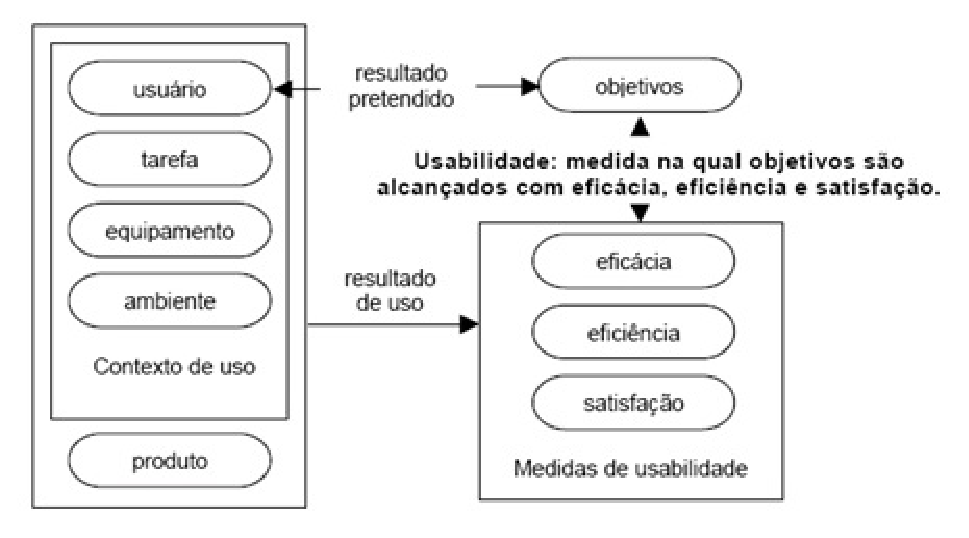
\includegraphics[keepaspectratio=true,scale=0.60]
      {figuras/estruturausabilidade9241.eps}
    \caption{Estrutura de Usabilidade Norma ISO 9241~\cite{cybis2010ergonomia}}
    \label{tdd_ciclo}
\end{figure}

\subsection{Interação Humano Computador}

	O Termo Human Computer Interaction  (HCI) começou a ser adotado na década de 1980 para descrever uma nova área de estudo na qual se preocupavam em saber como o uso dos computadores poderia enriquecer a vida pessoal e profissional dos seus usuários. (Moraes, 2002). \\
	A interação humano computador tem o principal objetivo de melhorar a eficácia e proporcionar satisfação do usuário. Para Preece (1994), o objetivo do HCI são desenvolver e aprimorar sistemas computacionais nos quais os usuários possam executar tarefas com segurança, eficiência e satisfação.

	
\subsection{Arquitetura da Informação}

A informação é algo que está presente no nosso dia-a-dia. Para (Wurman, 1991) a informação deve ser aquilo que leva à compreensão. A quantidade de conteúdo que é produzido na internet extrapola a capacidade humana de retenção da informação. (Santa Rosa). Esse excesso de informação contribui para o aumento dos problemas de usabilidade e da necessidade de pesquisa na área de interação humano-computador. (Agner, 2004).\\

Segundo Garrett (2003), a arquitetura da informação são a arte e a ciência de estruturar e organizar os ambientes informacionais para ajudar as pessoas a encontrarem e administrarem informações.\\

O arquiteto de informação deve ser um profissional multidisciplinar com conhecimentos em design gráfico, ciência da informação, biblioteconomia, jornalismo, engenharia de usabilidade, marketing e ciência da computação. Ele deve balancear as necessidades do usuário com os objetivos do negócio. (Rosenfeld e Morville, 1998).

\subsection{Ergonomia}

A ergonomia está na origem da usabilidade, pois visa proporcionar eficácia e eficiência, além de bem-estar e saúde do usuário através da adaptação do trabalho ao homem. O seu objetivo é garantir que sistemas e dispositivos estejam adaptados às maneiras de pensar, agir e trabalhar do usuário. ~\cite{cybis2010ergonomia}


\subsection{Engenharia de Usabilidade}

A engenharia de usabilidade surgiu no final dos anos 80 com o esforço sistemático das empresas e organizações para desenvolver programas de software interativo com usabilidade. Sua origem parte de iniciativas de cientistas como Card, Moran e Newell (Modelo do processador Humano de 1983) e Norman (Teoria da Ação de 1989). O objetivo era produzir conhecimentos que favorecesse a concepção de interfaces humano-computador mais adaptadas. ~\cite{cybis2010ergonomia}
\\
Podemos fazer um paralelo da engenharia de usabilidade com a engenharia de software. A engenharia de software ocupa do desenvolvimento do núcleo funcional de um sistema interativo formado por estruturas de dados, algoritmos e recursos de processamento de dados. Esse núcleo é construído de forma que o sistema funcione bem, de forma correta, rápida e sem erros. Já a engenharia de usabilidade ocupa-se da interface com o usuário que interliga as funções do sistema com os usuários de forma que a interface do sistema seja agradável, intuitivo, eficiente e fácil de operar.~\cite{cybis2010ergonomia}

\subsubsection{Ciclo de Engenharia de Usabilidade}

	O ciclo foi definido sendo essencialmente evolutivo, interativo e baseado no envolvimento do usuário. A norma ISO 13407 (Projeto centrado no usuário) sugere quatro principais etapas desse ciclo (analisar e especificar o contexto de operação; especificar as exigências dos usuários e organizações; produzir soluções de projeto; avaliar o projeto contra as exigências). ~\cite{cybis2010ergonomia}

Colocar figura: Projeto centrado no usuário

\subsection{Experiência do Usuário - UX}
É toda a interação que temos com um produto, serviço ou marca.
UX é um termo usado frequentemente para sintetizar toda a experiência com um produto de software. Não engloba  somente nas funcionalidades (Travis)

%Verificar as leituras

\subsection{Relação de todas essas áreas com a Usabilidade}

\section{A importância e os benefícios da Usabilidade}

No modo geral, os projetistas sabem da importância de desenvolver com enfoque no usuário e na usabilidade, mas normalmente os projetos são desenvolvidos sem que tenham sido realizadas pesquisas e aplicados métodos e técnicas de usabilidade.
	
	O tempo e os recursos limitados são as principais razões que impede a implatação dos testes de usabilidade nas equipes de software. Também há o desconhecimento por parte da equipe de desenvolvimento das técnicas a serem empregadas.

Incorporar a usabilidade no seu processo pode reduzir os custos e tempo de desenvolvimento e melhorar o produto final. Ter em mente  em quem é o usuário final em todas as etapas de desenvolvimento e processos de produção, desde análise das necessidades e projeto conceitual até prototipagem e produção.  (reescrever)

	O investimento na área de usabilidade agrega valor ao produto e traz beneficios não somente aos usuários, mas também aos seus produtores. 

Para a Associação de Profissionais de usabilidade (UPA), a usabilidade inclui os seguintes benefícios:

\begin{itemize}
\item Aumentar a produtividade
\item Diminuir custos de treinamento e suporte
\item Aumentar as vendas e as revendas
\item Reduzir os custos de desenvolvimento e manutenção.
\item Aumentar a satisfação do consumidor.
\end{itemize}


\section{Design Centrado no usuário}

É um processo de criação que se baseia nas necessidades, desejos e limitações das pessoas. O usuário deve está presente no ínicio ao fim do projeto.
O DCU deve-se iniciar com usuários e suas necessidades em vez de começar com a tecnologia.
O DCU surgiu da IHC e consiste em uma metodologia de design de software para 

%	Detalhar o fluxo do DCU

Para criar produtos que os usuário amem, é necessário incluir os usuários no processo de criação dos produtos (Travis Lowrdemilk)

\section{Métodos Agéis e o DCU}

\subsection{O ciclo da engenharia de usabilidade e as abordagens para o desenvolvimento de software}

	Exitem 2 grandes abordagens para o desenvolvimento de software: A abordagem tradicional sendo o seu principal método o (RUP - Rational Unified Process) e a abordagem ágil.
	Nesse trabalho iremos abordar somente os métodos ágeis de desenvolvimento de software que é o principal método utilizado no desenvolvimento de software livre atualmente.

Explicar os métodos àgeis

Citar manifesto ágil

As características da abordagem ágil facilitam na utilização da ergonomia e da usabilidade durante o desenvolvimento de software, mas os ergonomistas e engenheiros de usabilidade deverão adaptar suas técnicas de análise, modelagem, projeto e teste adotando-se os preceitos do manifesto ágil. (Cybis)

\begin{itemize}
\item Modelagem e projeto de interfaces devem ser orientados a padrões de projeto.
\item As avaliações de ergonomia, testes de usabilidade e especificações de revisões de interface devem ser realizados rapidamente.
\end{itemize}

Citar a filosofia de trabalho que a  ISO 13407 define para as empresas que vise a usabilidade.

Modelos de Ciclo de Vida

	Para que possamos conhecer o processo completo de desenvolvimento é importante considerar as como as atividades se relacionam. Entender que atividades estão envolvidas no design de interação é o primeiro passo para estar apto à faze-lo.
	O termo modelo de ciclo de vida é utilizado para representar um modelo que capta um conjunto de atividades e a maneira como elas se relacionam. ~\cite{preece2005interacao}

	Existe alguns modelos de processo de engenharia de usabilidade:

\begin{itemize}
\item Projeto Centrado no Usuário da Norma ISO/IEC 13407
\item Modelo Estrela
\item Ciclo de vida de Engenharia de Usabilidade
\end{itemize}


O ciclo de vida da Engenharia de Usabilidade

	
	O ciclo de vida de engenharia de usabilidade foi proposto por Deborah Mayhew em 1999. 
A ISO 13407 também propõe um modelo de ciclo de concepção centrado no usuário. Ambos possuem a mesma estrutura e propõem ciclos de atividades de análise, projeto, construção e testes. ~\cite{cybis2010ergonomia}

	O ciclo proposto por Mayhew oferece uma visão holística acerca dessa engenharia e uma descrição detalhada de como podemos realizar os testes de usabilidade (PREECE).

A. Análise de Requisitos

	Mayhew propõe quatro tipos de atividades de análise de requisitos: 

\begin{itemize}
\item Análise do perfil do usuário
\item Análise do contexto da tarefa
\item Análise das possibilidades e restrições da plataforma
\item Análise dos princípios gerais para o projeto
\end{itemize}

	Depois da análise dos requisitos é preciso especificar as metas de usabilidade do futuro sistema. A norma ISO 9241:11 orienta como podemos especificar essas metas

B. Projeto, Testes e Implementação

	

C. Instalação



